\documentclass{article}[12pt]
\renewcommand{\baselinestretch}{1.5}

\usepackage[parfill]{parskip}
\usepackage[affil-it]{authblk}
\usepackage[space]{grffile}

\usepackage[a4paper]{geometry}
\geometry{verbose}
\usepackage{float}
\usepackage{graphicx}
\usepackage{setspace}
\usepackage{caption}

\usepackage[utf8]{inputenc}
\usepackage[english]{babel}

\usepackage{latexsym,textcomp,longtable,tabulary}
\usepackage{booktabs,array,multirow}
\usepackage{amsfonts,amsmath,amssymb,mathbbol,calc}
\usepackage{subfigure,color,blindtext,enumitem,siunitx}

\usepackage{mathtools}
\usepackage{url,hyperref,etoolbox}
\numberwithin{equation}{section}
\hypersetup{colorlinks=false,pdfborder={0 0 0}}

%+figure layout options
\restylefloat{figure}
\setlist{leftmargin=*,before=\setlength{\rightmargin}{\leftmargin}}
%-figure layout options

\providecommand\citet{\cite}
\providecommand\citep{\cite}
\providecommand\citealt{\cite}

\setlength{\parskip}{1em}
\makeatletter
\makeatother


\newif\iflatexml\latexmlfalse
\providecommand{\tightlist}{\setlength{\itemsep}{0pt}\setlength{\parskip}{0pt}}%
\AtBeginDocument{\DeclareGraphicsExtensions{.pdf,.PDF,.eps,.EPS,.png,.PNG,.tif,.TIF,.jpg,.JPG,.jpeg,.JPEG}}
\begin{document}

\title{
On the affect of the Laplacian in equlibration\\
dynamics of the Spherical Model
}

\author{Gregory Szep}
\affil{King's College London}
\date{\today}
\maketitle

\section{Mathematical Analysis}
\vspace{-10pt}
\subsection{Motivation for the Model}
Consider $N$ nodes in a undirected network passing around a finite resource.
Eventually the resource will equilibrate within the network solely due it its
finiteness. We wish to study the equilibration timescales of such a problem,
where finiteness of the resource and connectedness of the network may be
expressed is a variety of ways, giving rise different flavours of the
Sherrington-Kirkpatrick spherical model.

Exact dynamical solutions can be obtained if finiteness of the resource
is the expressed as a constant $L_2$ norm across all the nodes. In addition,
if the connectedness of the network is known, it may be used to obtain explicit
expressions --- at least in some limit --- for the dynamics of the resource,
and hence timescales can be extracted.

The Wigner ensemble is used to generate the connectivity in an attempt to
minimise a priori assumptions on it. Then intorducing the $M$-dimensional
periodic lattice laplacian allows the study of the model as it departs from
randomness and gains spatial structure. Is it possible to extract the dimension
of the manifold that the nodes lie on simply from observed correlations and
equilibration timescales in the resource? This work may have applications in
dimensionality reduction methods.

\subsection{Analytical Solution of the Langevin Equation}
Let the resource across $N$ nodes be represented by vector $s(t)\in\mathbb{R}^N$,
and the weighted undirected connections between them be a Hermitian $N\times N$ matrix
$\mathbf{J}$. This matrix represents the rate at which the resource is passed between
nodes. Without finiteness, we can solve the linear equations, revealing that
the resource at different nodes would diverge or go to zero depending on the sign
of the eigenvalues of $\mathbf{J}$. This does not seem reasonable.

Therefore a lagrange multiplier $\mu(t)\in\mathbb{R}$ is introduced which holds
the $L_2$ norm of vector $s(t)$ constant. This implicitly introduces a nonlinearity.
The dynamics is cast as a Langevin Equation with white noise $\xi(t)\in\mathbb{R}^N$
which is characterised by its moments $\langle\dots\rangle$. Eventually the resource
will equilibrate due it its finiteness, subject to the amplitude of the noise.
The symbol $\mathbb{1}$ represents the diagonal identity.
\begin{align}
  \partial_t s = \big[\mathbf{J}-\mathbb{1}\mu(t)\big]s+\xi
\end{align}
\vspace{-40pt}
\begin{align}
  \left\langle\xi(t)\right\rangle=\mathbb{0}\qquad
  \left\langle\xi(t)\xi(t')\right\rangle=2T\mathbb{1}\delta(t-t')
\end{align}
\vspace{-40pt}
\begin{align}
\text{where}\quad\mu(t) = \frac{1}{N}s^{\top}\left(\mathbf{J}s+\xi\right)
\quad\text{enforces constraint}\quad|s(t)|^2=N
\label{eq:constraint}
\end{align}
It is possible to solve the inhomogenous time-dependent ordinary linear system of
differential equations for $s(t)$ using integrating factor method and rotate
into the eigenbasis $\sigma_{\lambda}(t)\in\mathbb{R}$ of matrix $\mathbf{J}$. This does not
yield a closed form for $\mu(t)$ however; the derivation by Cugliandolo, L. F.
and Dean D. S.~\cite{} yields the moments below for the uniform
initial condition $\sigma_{\lambda}(0)=1$. Here the complexity lies in performing
the inverse laplace transform $\mathcal{L}^{-1}$ which in turn depends on the
eigenvalue distribution $p(\lambda\in\mathbf{J})$.
\begin{align}
  \langle \sigma_{\lambda}(t)\rangle=
    \frac{\mathbb{e}^{\lambda t}}{\sqrt{\Gamma(t)}}\qquad
  \langle \sigma_{\lambda}(t)\sigma_{\lambda'}(t')\rangle=
\end{align}
\vspace{-30pt}
\begin{align}
  \Gamma(t)=
    \sum_{k=0}^{\infty}(2T)^k
    \mathcal{L}^{-1}\left[\Phi(s)^k\right]\quad\text{where}
    \quad
    \Phi(s)=\int\frac{p(\lambda\in\mathbf{J})}{s-2\lambda}\mathrm{d}\lambda
    \label{eq:gamma}
\end{align}
\pagebreak
\subsection{Hermitian Wigner Ensemble}
Suppose the connections between nodes are given by a random matrix
$\mathbf{H}$ taken from the Hermitian Wigner ensemble, whos upper triangle elements
$[\mathbf{H}]_{ij}$ are distributed according to a density $\mathbb{P}$ with
subexponential tails~\cite{} with expectation $\mathbb{E}$ and variance
$\mathbb{V}$, such that in the limit $N\rightarrow\infty$ the eigenvalue
spectrum converges to the semicircle law $p(\lambda\in\mathbf{H})\rightarrow\cap(\lambda|J)$.
Below the symbols $\mathbf{0}$ and $\mathbf{1}$ denote constant matrices of zeros and ones
respectively.
\begin{align}
\cap(\lambda|J)=\frac{1}{2\pi J^2}\sqrt{4J^2-\lambda^2}\label{eq:semicircle}
\quad\quad\\
\mathbb{E}[\mathbf{H}]=\mathbf{0}
\quad
\mathbb{V}[\mathbf{H}]=\frac{J^2}{N}(\mathbf{1}+\mathbb{1})
\quad\\
\mathbb{P}\left(
t^\alpha\leq
\left|[\mathbf{H}]_{ij}\right|
\right)\leq e^{-t}
\quad
\forall t\geq\alpha,\forall i,j
\end{align}
To match the terms of the expansion in~(\ref{eq:gamma}) to known inverse laplace
transforms some algebraic trickery is required: after substituting the limiting
density~(\ref{eq:semicircle}) into the second equation in~(\ref{eq:gamma}) the
infinite sum is evaluated first. Then the result is expanded in terms the denominator
part that is a function of $s$. Only then do the terms match the laplace transforms
of modified Bessel functions of the first kind $\frac{I_{l}(4Jt)}{t}$.
These have well-known asymtotics for $z\rightarrow\infty$
\begin{align}
  \Phi(s)=\frac{s-\sqrt{s^2-16J^2}}{8J^2}\qquad
  \Gamma(t)=\frac{1}{2T}
  \sum_{l=1}^{\infty}l\left(\frac{T}{J}\right)^{l}\frac{I_{l}(4Jt)}{t}
\end{align}
\pagebreak
\subsection{Discrete Laplacians}
Using the Circular Diagonalization Theorem~\cite{} one can derive the
eigenvalues $\lambda_N(k)$ of an $N\times N$ matrix $\mathbf X$ which
represents the second-order central difference approximation to the
second derivative along $N$ sites of a one dimensional ring.
\begin{align}
  \mathbf X :=
  \begin{pmatrix}
    -2 & 1 &  &  &  & 1 \\
    1 & -2 & 1 &  &  &  \\
    & 1 & \ddots & \ddots &  & \\
    & & \ddots & \ddots & 1 & \\
    & & & 1 & -2 & 1 \\
    1 & & & & 1 & -2 \\
  \end{pmatrix}\\
  \begin{matrix}
    \lambda_N(k)=2\left(\cos\left(\frac{2\pi k}{N}\right)-1\right) \\
    k\in\{0,1,\cdots,N-1\}
  \end{matrix}
  \qquad
\end{align}
As the number of sites $N\rightarrow\infty$ the argument $k/N\in[0,1]$
and the eigenvalues remain bounded $-2<\lambda<0$. By shifting and scaling
the index $k\rightarrow\frac{k-N\pi}{2\pi}$ the eigenvalues are expressed as
the familiar dispersion relation~\cite{}.
\begin{align}
  \lambda(x)&=
  -2\left(\cos x+1\right)
  \quad x\in[-\pi,\pi]
\end{align}
The discrete $M$-dimensional laplacian is simply the kronecker sum of one
dimensional cases $\mathbf\Delta=\mathbf X\oplus\mathbf X\oplus\cdots\oplus\mathbf X$
and thus its eigenvalues is simply the sum one dimensional dispersions~\cite{}.
\begin{align}
  \lambda(\bar{\mathbf{x}})&=
  -2\sum_{x\in\bar{\mathbf{x}}}\left(\cos x+1\right)
  \quad \bar{\mathbf{x}}\in[-\pi,\pi]^M
\end{align}
The probability density $\Delta_M(\lambda)$ can be expressed as an integral
over the $M$-dimensional hypercube region $\Omega=[-\pi,\pi]^M$ in complete
analogue with the density of states.
\begin{align}
  \Delta_M(\lambda')&=\frac{1}{Z_M}\int_{\Omega}\!\delta(\lambda'-\lambda(\bar{\mathbf{x}}))\,\mathrm{d}\bar{\mathbf{x}}
\end{align}
We proceed with an element-wise change of variables $\bar{\mathbf{u}}=2\cos \bar{\mathbf{x}}$ and
recognise that the integration region is $M$-fold symmetric across each
component axis, which allows restriction of the domain of integration to a
hyperoctant. In coordinates $\bar{\mathbf{u}}$ the region becomes $\Omega'=[-2,2]^M$.

\begin{align*}
  \Delta_M(\lambda)&=\frac{1}{Z_M}
  \int_{\Omega'}\!
  \frac{\delta(\Lambda_M+\sum_{u\in\bar{\mathbf{u}}}u)}
  {\sqrt{\prod_{u\in\bar{\mathbf{u}}}(1-u^2/4) }}
  \,\mathrm{d}\bar{\mathbf{u}}
  \qquad
  \begin{matrix}
    \Lambda_M=\lambda+2M \\
    |\Lambda_M|\leq2M
  \end{matrix}\\
  &=\frac{1}{2\pi Z_M}
  \int_{-\infty}^{\infty}\int_{\Omega'}\!
  \frac{\mathbb{e}^{\Lambda_M\mathbb{i}k}\exp[\sum_{u\in\bar{\mathbf{u}}}u\mathbb{i}k]}
  {\sqrt{\prod_{u\in\bar{\mathbf{u}}}(1-u^2/4) }}
  \,\mathrm{d}\bar{\mathbf{u}}\mathrm{d}k\\
  &=\frac{1}{2\pi Z_M}
  \int_{-\infty}^{\infty}\mathbb{e}^{\Lambda_M\mathbb{i}k}
  \prod_{u\in\bar{\mathbf{u}}}\int_{-2}^{2}\!
  \frac{\mathbb{e}^{u\mathbb{i}k}}
  {\sqrt{1-u^2/4}}
  \,\mathrm{d}u\mathrm{d}k
\end{align*}
The fourier representation of the delta function allowed the
factorisation of the integral. We recognise a repeated Bessel
integral and replace it with the Bessel function of the first kind
$J_n(k)$, leaving only a fourier transform which we define
$ \mathcal{F} :
f\rightarrow \frac{1}{\sqrt{2\pi}}
\int_{-\infty}^{\infty}f(k)e^{\mathbb{i}\Lambda k}\mathrm{d}k$. To clean
the formula up even further we may use the convolution
theorem to deal with the powers of $M$, leaving only the fourier
transform of the Bessel function $J_0(k)$, which is the arcsine
distribution $\alpha(\lambda)$. It becomes clear that the eigenvalue
density of a kronecker sum of matrices is the convolution of the densities
of those matrices.
\begin{align}
  \Delta_M(\lambda)=\underbrace{
  \alpha(\lambda)*\alpha(\lambda)*\cdots*\alpha(\lambda)}_{M}\qquad\qquad\qquad\\
  \begin{matrix}
    \alpha(\lambda)=
      \frac{1}{2\pi\sqrt{1-\left(\frac{\lambda+2}{2}\right)^2}}
      \Pi\left(\frac{\lambda+2}{2}\right)
    &&
    \Pi(x)=
      \begin{cases}
        1 & |x|<1\\
        0 & |x|\geq1\\
      \end{cases}
  \end{matrix}
  \label{eq:arcsine}
\end{align}
\begin{figure}[H]
\centering{}
\captionsetup{justification=centering}
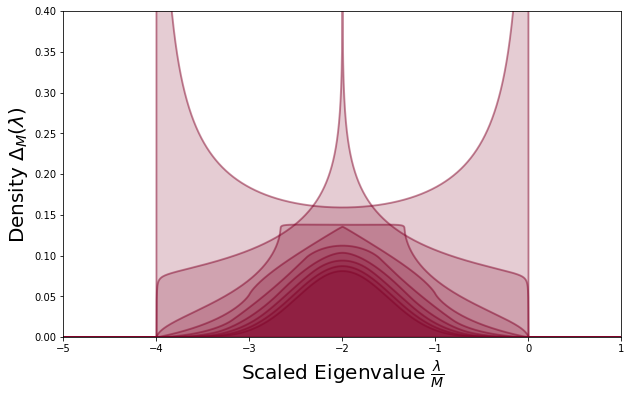
\includegraphics[scale=0.45]{figures/density}
\caption{Eigenvalue distributions $\Delta_M(\lambda)$ of the $M$-dimensional Laplacian}
\label{fig:dos}
\end{figure}
The one dimensional density has two Van Hove singularities at $\lambda=-4,0$
given by the arcsine law $\alpha(\lambda)$, whereas the two dimensional
case has one at $\lambda=-4$ given by the complete elliptic integral
of the first kind $K(m)$. Figure~\ref{fig:dos} reveals that in higher
dimensions singularities do not occur; instead there appear to be
discontinuities in the higher order derivatives. The density smooths out
as repeated convolutions bring it to a normal distrubtion; this is another
way to state the Central Limit Theorem~\cite{}.

Substituting the limiting density~(\ref{eq:arcsine}) into the second equation
in~(\ref{eq:gamma}) the inverse laplace transform of the powers can be
performed immediately.
\begin{align}
  \Phi(s)=\frac{1}{\sqrt{8s + s^2}}
  \qquad
  \Gamma(t)=2Te^{-4t}
  \sum_{k=0}^{\infty}\frac{(2Tt)^{k-1}}{(k-1)!}
  {}_0F_1(\frac{1+k}{2},4t^2)
\end{align}
\subsection{Sum of the Wigner and Laplacian Matrices}
In the formalism of Free Probability it is possible to express the
$N\rightarrow\infty$ limiting eigenvalue density $\rho$ of a sum of
matrices in terms of the free convolutions $[]$ the individual limiting
densities, provided that these densities have compact support~\cite{}.
The following expressions for the free convolution of a semicircle distrubtion
$\cap(\lambda|J)$ with an arbitrary compact distrubtion $\mu(\lambda)$ can be
used when one of these matrices comes from a Wigner Ensemble~\cite{Biane_1997}.
\begin{align}
  \mathcal{H}[\rho\circ\psi(\lambda|J)]=
  \int_{\mathbb{R}}\frac{(\lambda-\lambda')\mu(\lambda')\mathrm{d}\lambda'}{(\lambda-\lambda')^2+E(\lambda|J)^2}
  \qquad
  \psi(\lambda|J)=
  \lambda+J\mathcal{H}[\rho\circ\psi(\lambda|J)]
\end{align}
\vspace{-30pt}
\begin{align}
  E(\lambda|J)=\inf
  \left\{
  E\geq 0\,\,\bigg|\,
  \int_{\mathbb{R}}\frac{\mu(\lambda')\mathrm{d}\lambda'}{(\lambda-\lambda')^2+E^2}
  \leq\frac{1}{J}
  \right\}
\end{align}
\begin{figure}[H]
\centering{}
\captionsetup{justification=centering}
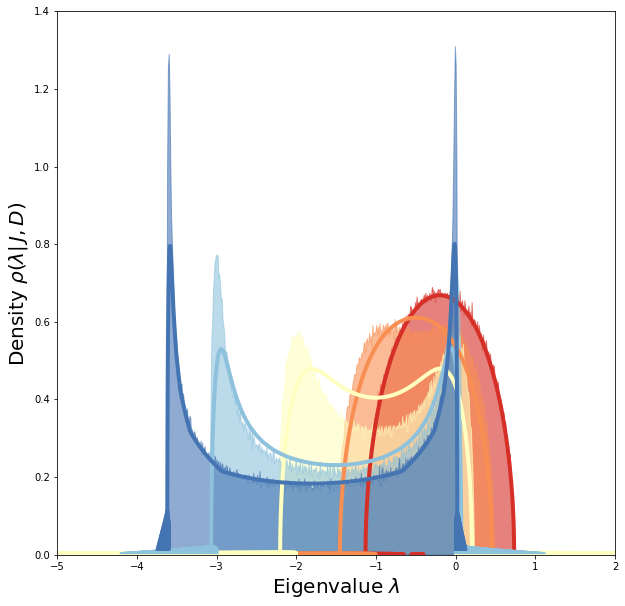
\includegraphics[scale=0.3]{figures/interaction1d}
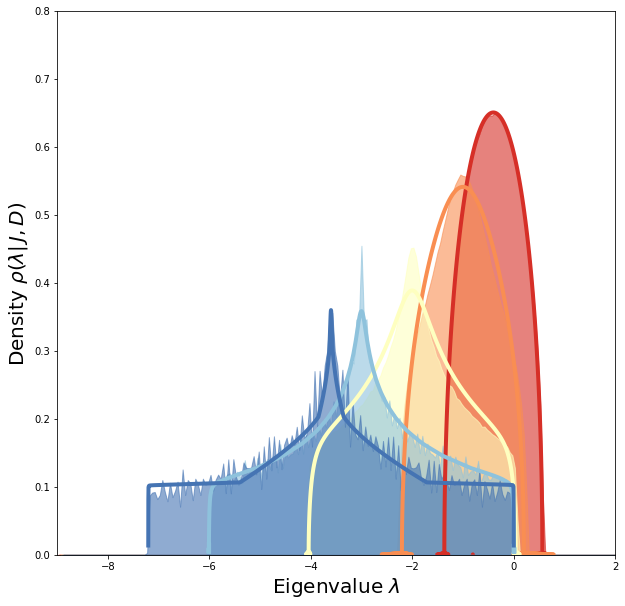
\includegraphics[scale=0.3]{figures/interaction2d}
\caption{Left/Right: Random interaction spectra $S(\lambda|\mu)$ for variable
values of the order parameter $\mu$ which introduces one/two dimensional laplacian}
\label{fig:spectrum}
\end{figure}

\bibliography{bibliography/biblio}
\bibliographystyle{ieeetr}
\end{document}
